\documentclass[12pt]{scrartcl}
\title{Assignment 3\\ Design Thinking:\\ Sketches and Wireframes}
\author{\textbf{Flow Overstack Team}\\ Cesana Filippo\\ Hartmann Kathrin\\ Gary\\ Rodolfo Masera Tommaso\\ Stucchi Jacopo\\ Taillefert Stefano}
\date{}
\setlength{\parindent}{0pt}

\usepackage{graphicx}
\usepackage{float}

\begin{document}

\maketitle

\tableofcontents

\newpage


\section{Introduction}

	Write a brief introduction referring back to your project and it basic concepts.

\section{Persona}

	% Describe briefly your design persona as distilled from the analysis of data gathered during Contextual Inquiry.
	
	The first task we went through was to summarize the interviews we conducted and extract meaningful data from all the kids' 
	answers to construct a user model for our application. The result is Kiddo, our design persona. Let us introduce him:\\
	
	Kiddo is the average 12-years-old, goes to middle school and loves spending time on his smartphone. He uses it mainly for 
	entertainment purposes, following his favorite youtubers and idols on social media, listening to music and chatting with his on- 
	and offline friends. Although its high affinity to his electronic device, our boy knows that he shouldn't exceed the usage limits 
	imposed by his parents and is well-aware that mobile phone addiction is just around the corner. For that reason, he doesn't
	stay on his phone for more than a couple of hours a day.\\
	
	He follows people like Footballo Socceri, the millionaire football player who likes to party and buy fast cars; 
	Trappino Trappisti, a rapper who rose to fame after punching a man on the street and whose songs are mainly violence-themed;
	Thotella DeThot, a TV showgirl widely known for her osé selfies posted on Instagram; and many others. Despite being interested 
	in their luxurious and cool lifestyle, Kiddo knows that they are not a good role model to follow; he is rather inspired by people
	who did something good for science, played a role in the history of humanity or left an important message for the future
	generations.\\
	
	Our persona doesn't dislike school, but he finds the ``classic" way of studying quite boring, bent over a textbook trying to memorize 
	dates and facts that he will forget in a couple of days anyway. In class, he often dreams of being somewhere else, learning 
	about something that \textit{really} amazes him. Kiddo thinks that there should be other ways of learning and that it should be
	more interactive.\\	
	
	\begin{figure}[H]
        		\centering
       		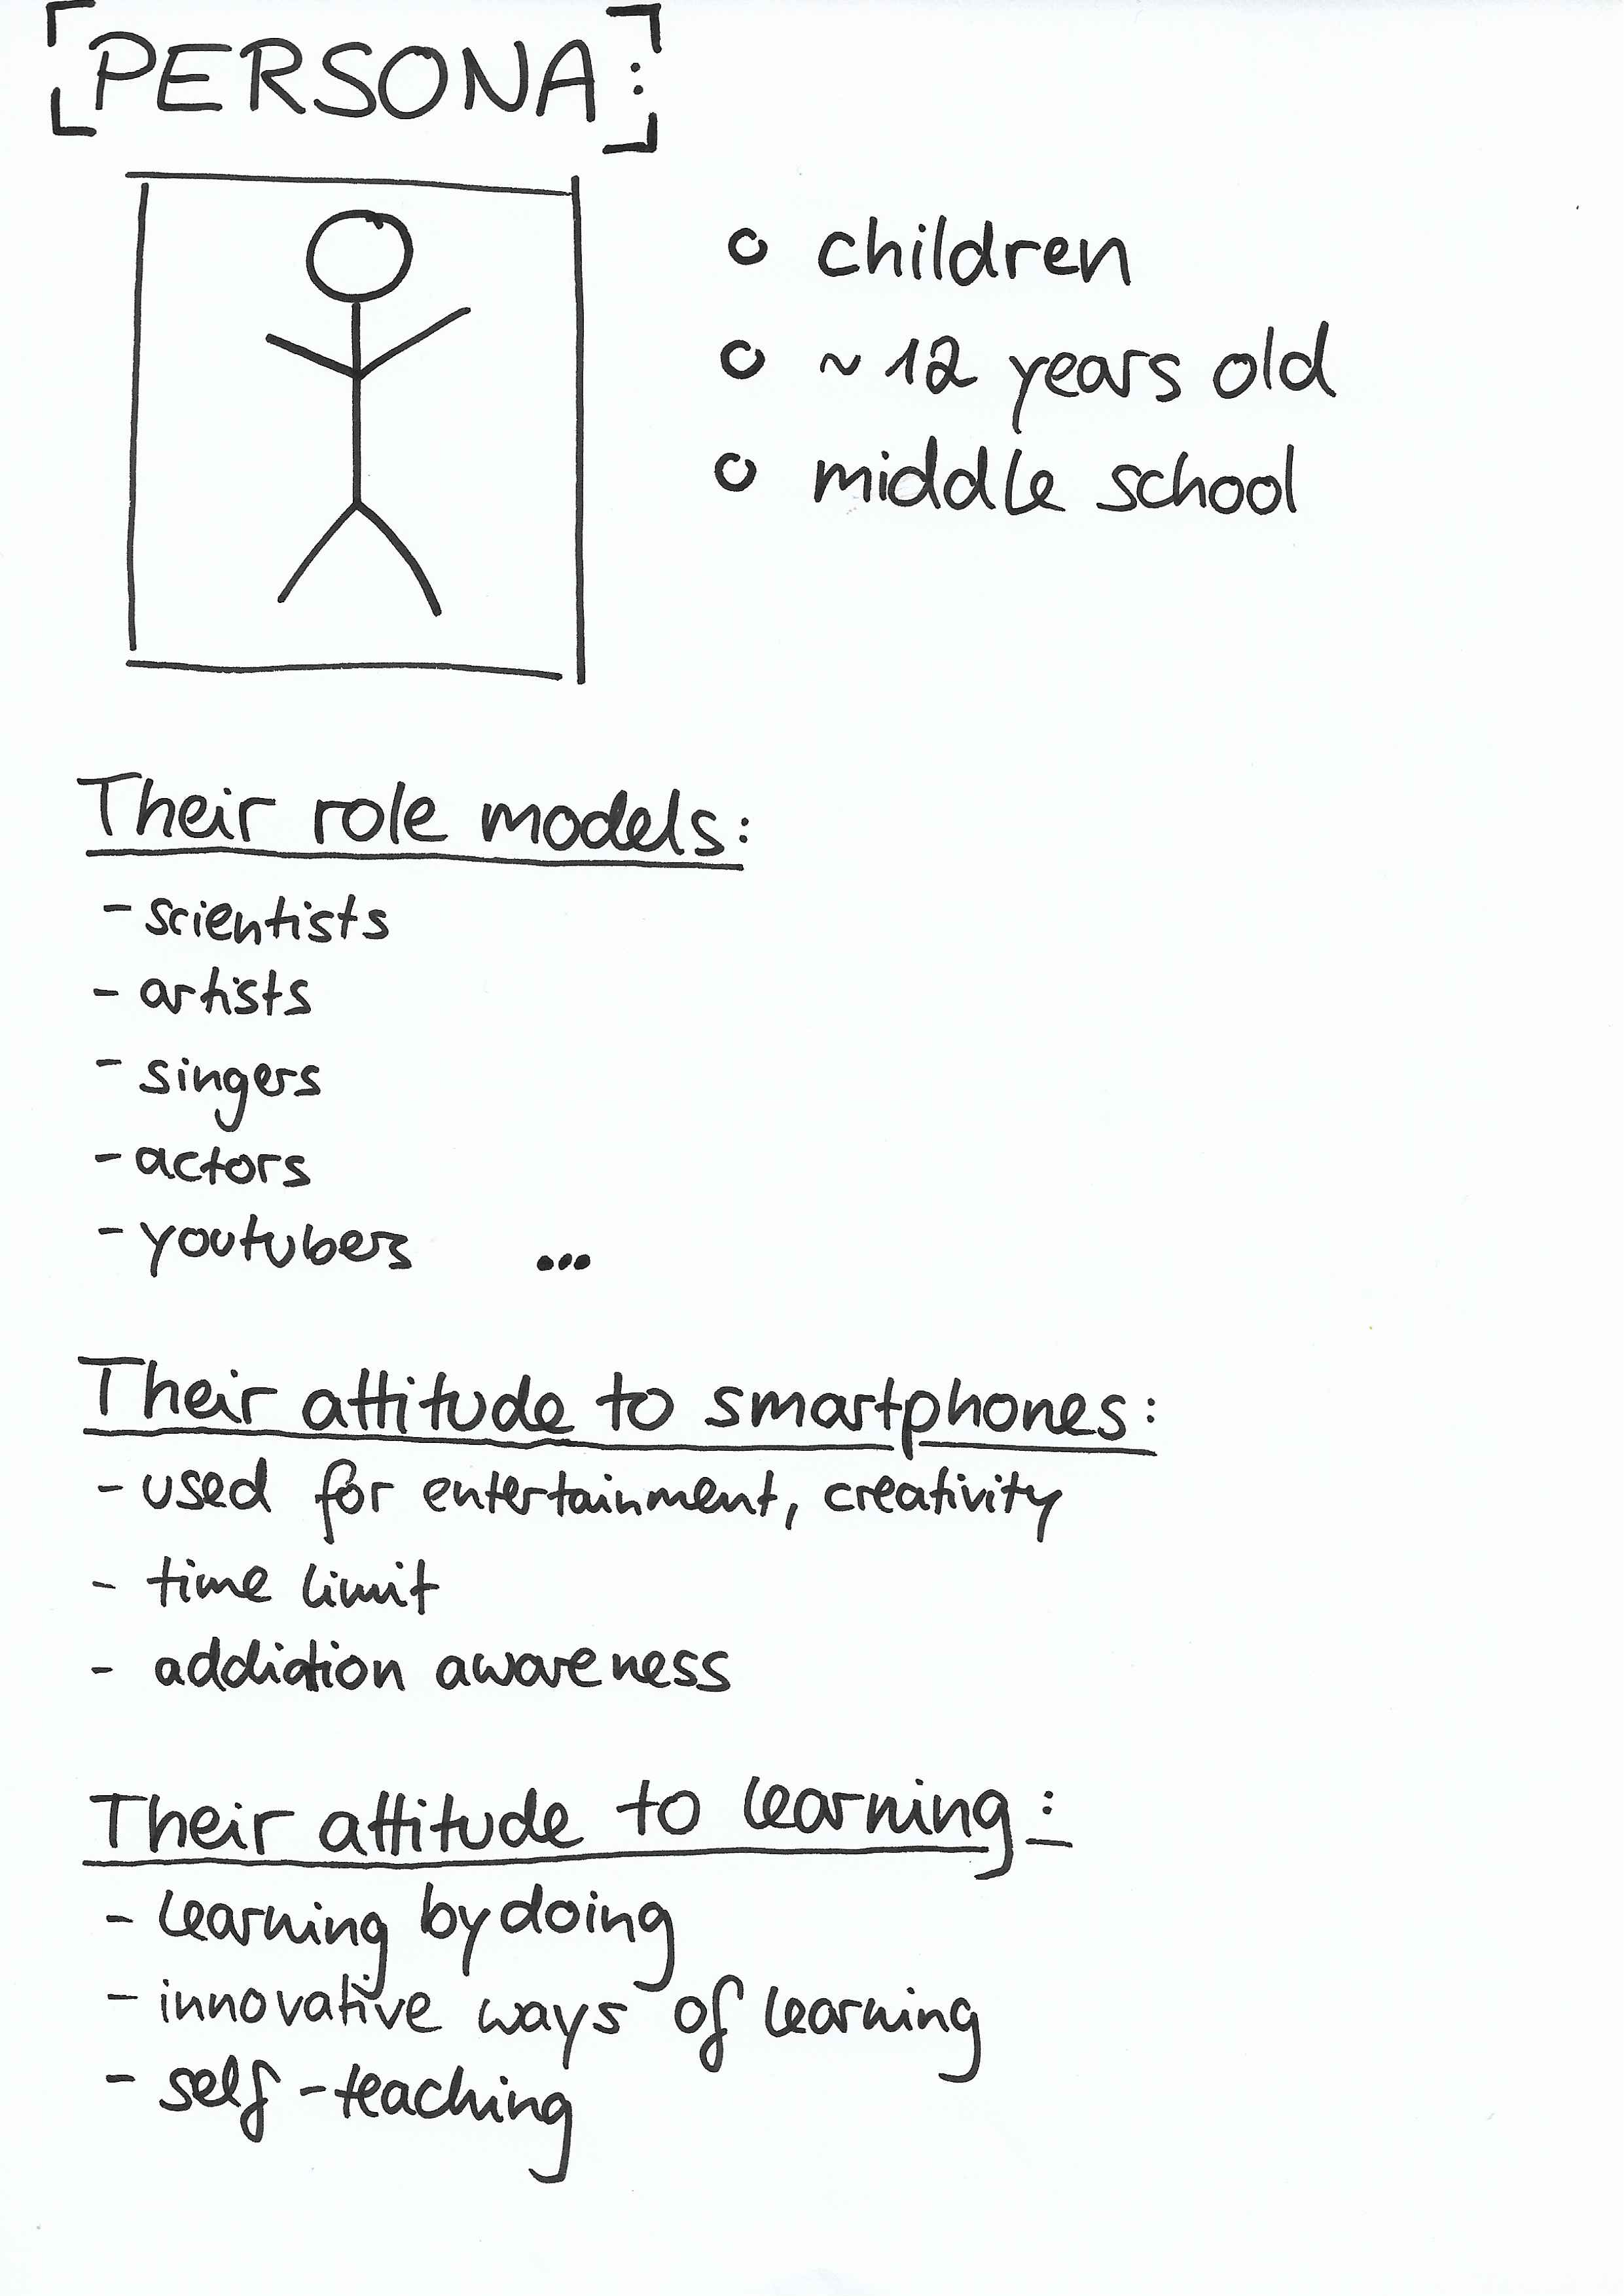
\includegraphics[width=\textwidth]{../images/persona.jpg}
       		\caption{Our persona draft}
        		\label{persona1}
	\end{figure}
	

\section{Ideation and sketching}

	Before being able to sketch a storyboard and a wireframe we had to identify the persona we 
	were going to design the application for. With that in mind we went over the data we gathered
	through the interviews.\\
	
	The ideation followed right after. As we reviewed our information we came up with and sketched 
	some storyboards depicting a possible situation which our users may find themselves in. 
	For instance, you could imagine a child wondering what they would want to be when they grow
	up; in such a situation our application may help a kid clear their mind or come up with something
	new they would want to check out.\\
	
	Other than the storyboards, we sketched the skeleton of a possible wireframe, which will be
	covered in more detail in its own section, but the main idea behind it is to make it, firstly,
	simple and intuitive. We do not wish for our users to feel overwhelmed or lost because of
	many unclear features; because of this, at this point in time, we opted for few and easy to
	understand mechanics, such as a feed, a camera button and menus for a personal profile and
	settings.\\
	
	To wrap it up, ideation and sketching took shape together as they complement each other for
	a successful early design. The ideation was a necessary step to sketch our ideas since we
	could not have drawn anything without first coming up with something to draw ourselves.
	Reviewing our data was the fundamental point of this step as we could not have proceeded
	otherwise.

\section{Workspace and materials}

	% Describe your workspace and the materials you used.
	Our workspace is basically a desk in the Informatics building, either in a class room or in the open space. The desk is mostly rectangular 
	but we sit around it as if it was King Arthur's round table. In that way, everybody can contribute his creative ideas. For drawing sketches, 
	designing storyboards and creating drafts, we go easy and plain: Paper and black pens are our fundamental material. 
	Colours are only used for highlighting and structuring.\\
	
	Apart from that, we use the walls in our class room to draft larger sketches. Drawing on the wall enables us from time to time to explain 
	complex ideas in a very easy way to our group members.
	
\section{Photos}

	% If appropriate, show photos of your team at work.
	
	\begin{figure}[H]
        		\centering
       		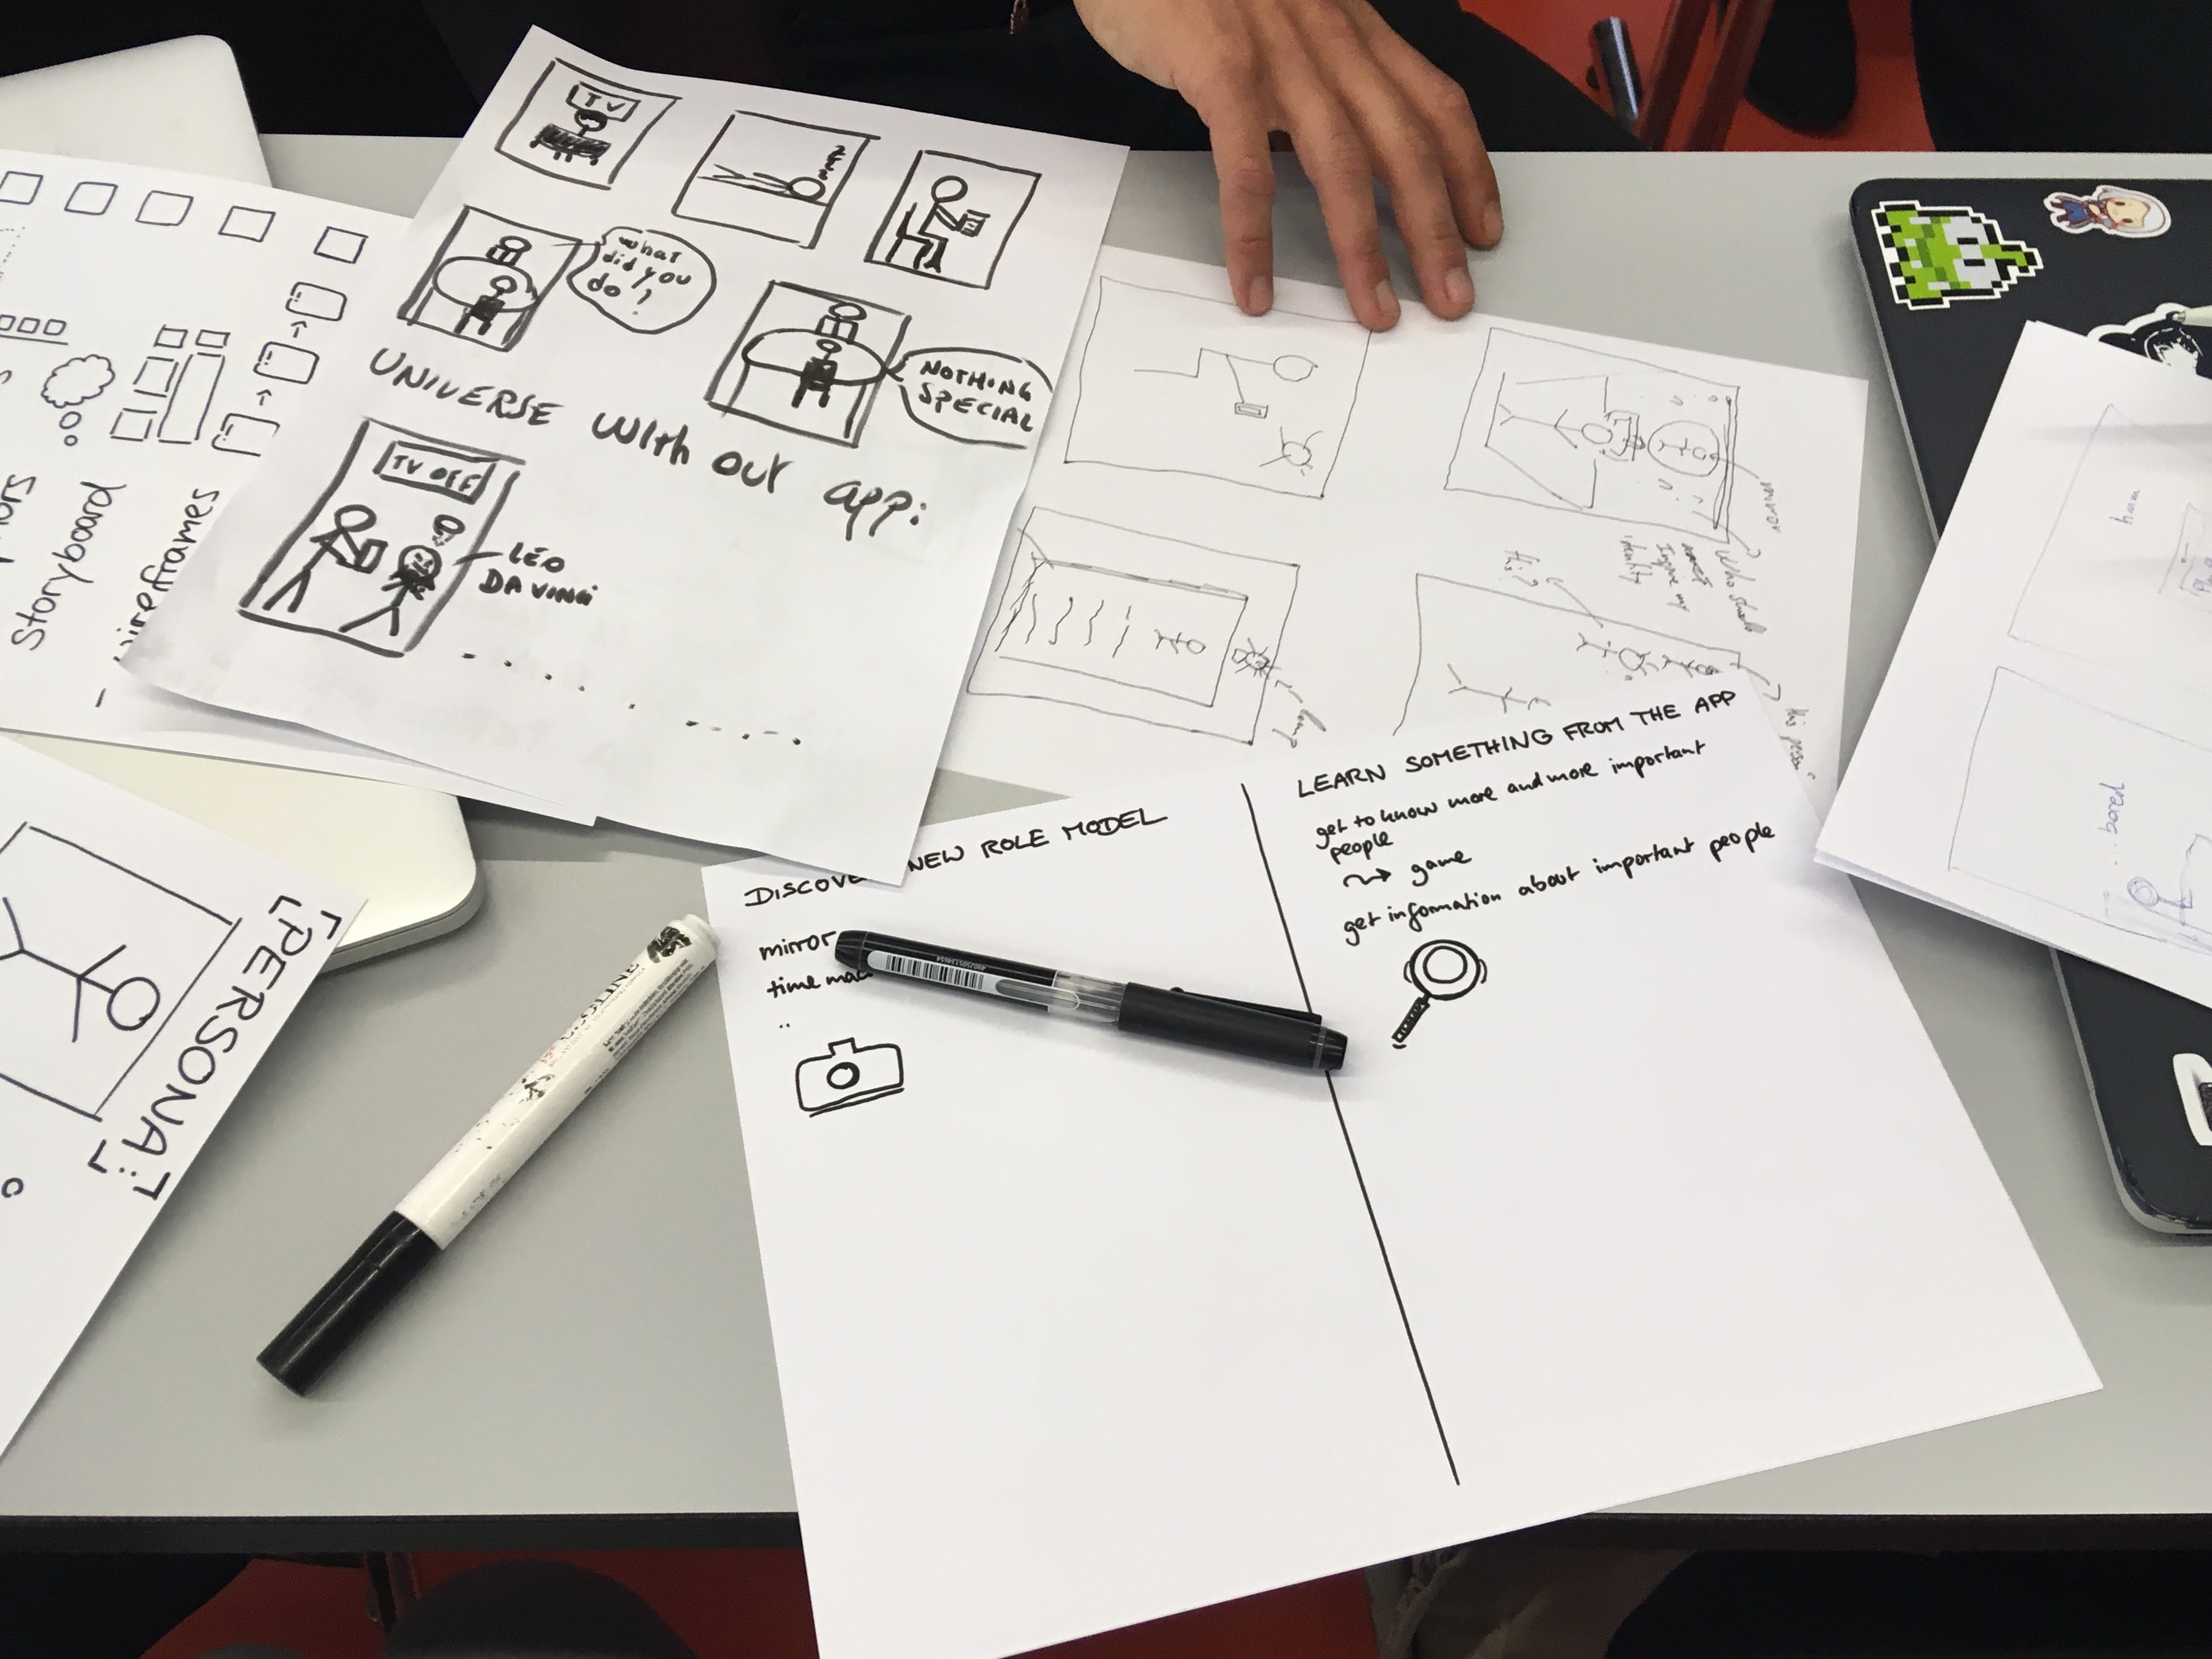
\includegraphics[width=\textwidth]{../images/group1.jpg}
       		\caption{Our creative sketching workspace}
        		\label{group1}
	\end{figure}
	
	\begin{figure}[H]
        		\centering
       		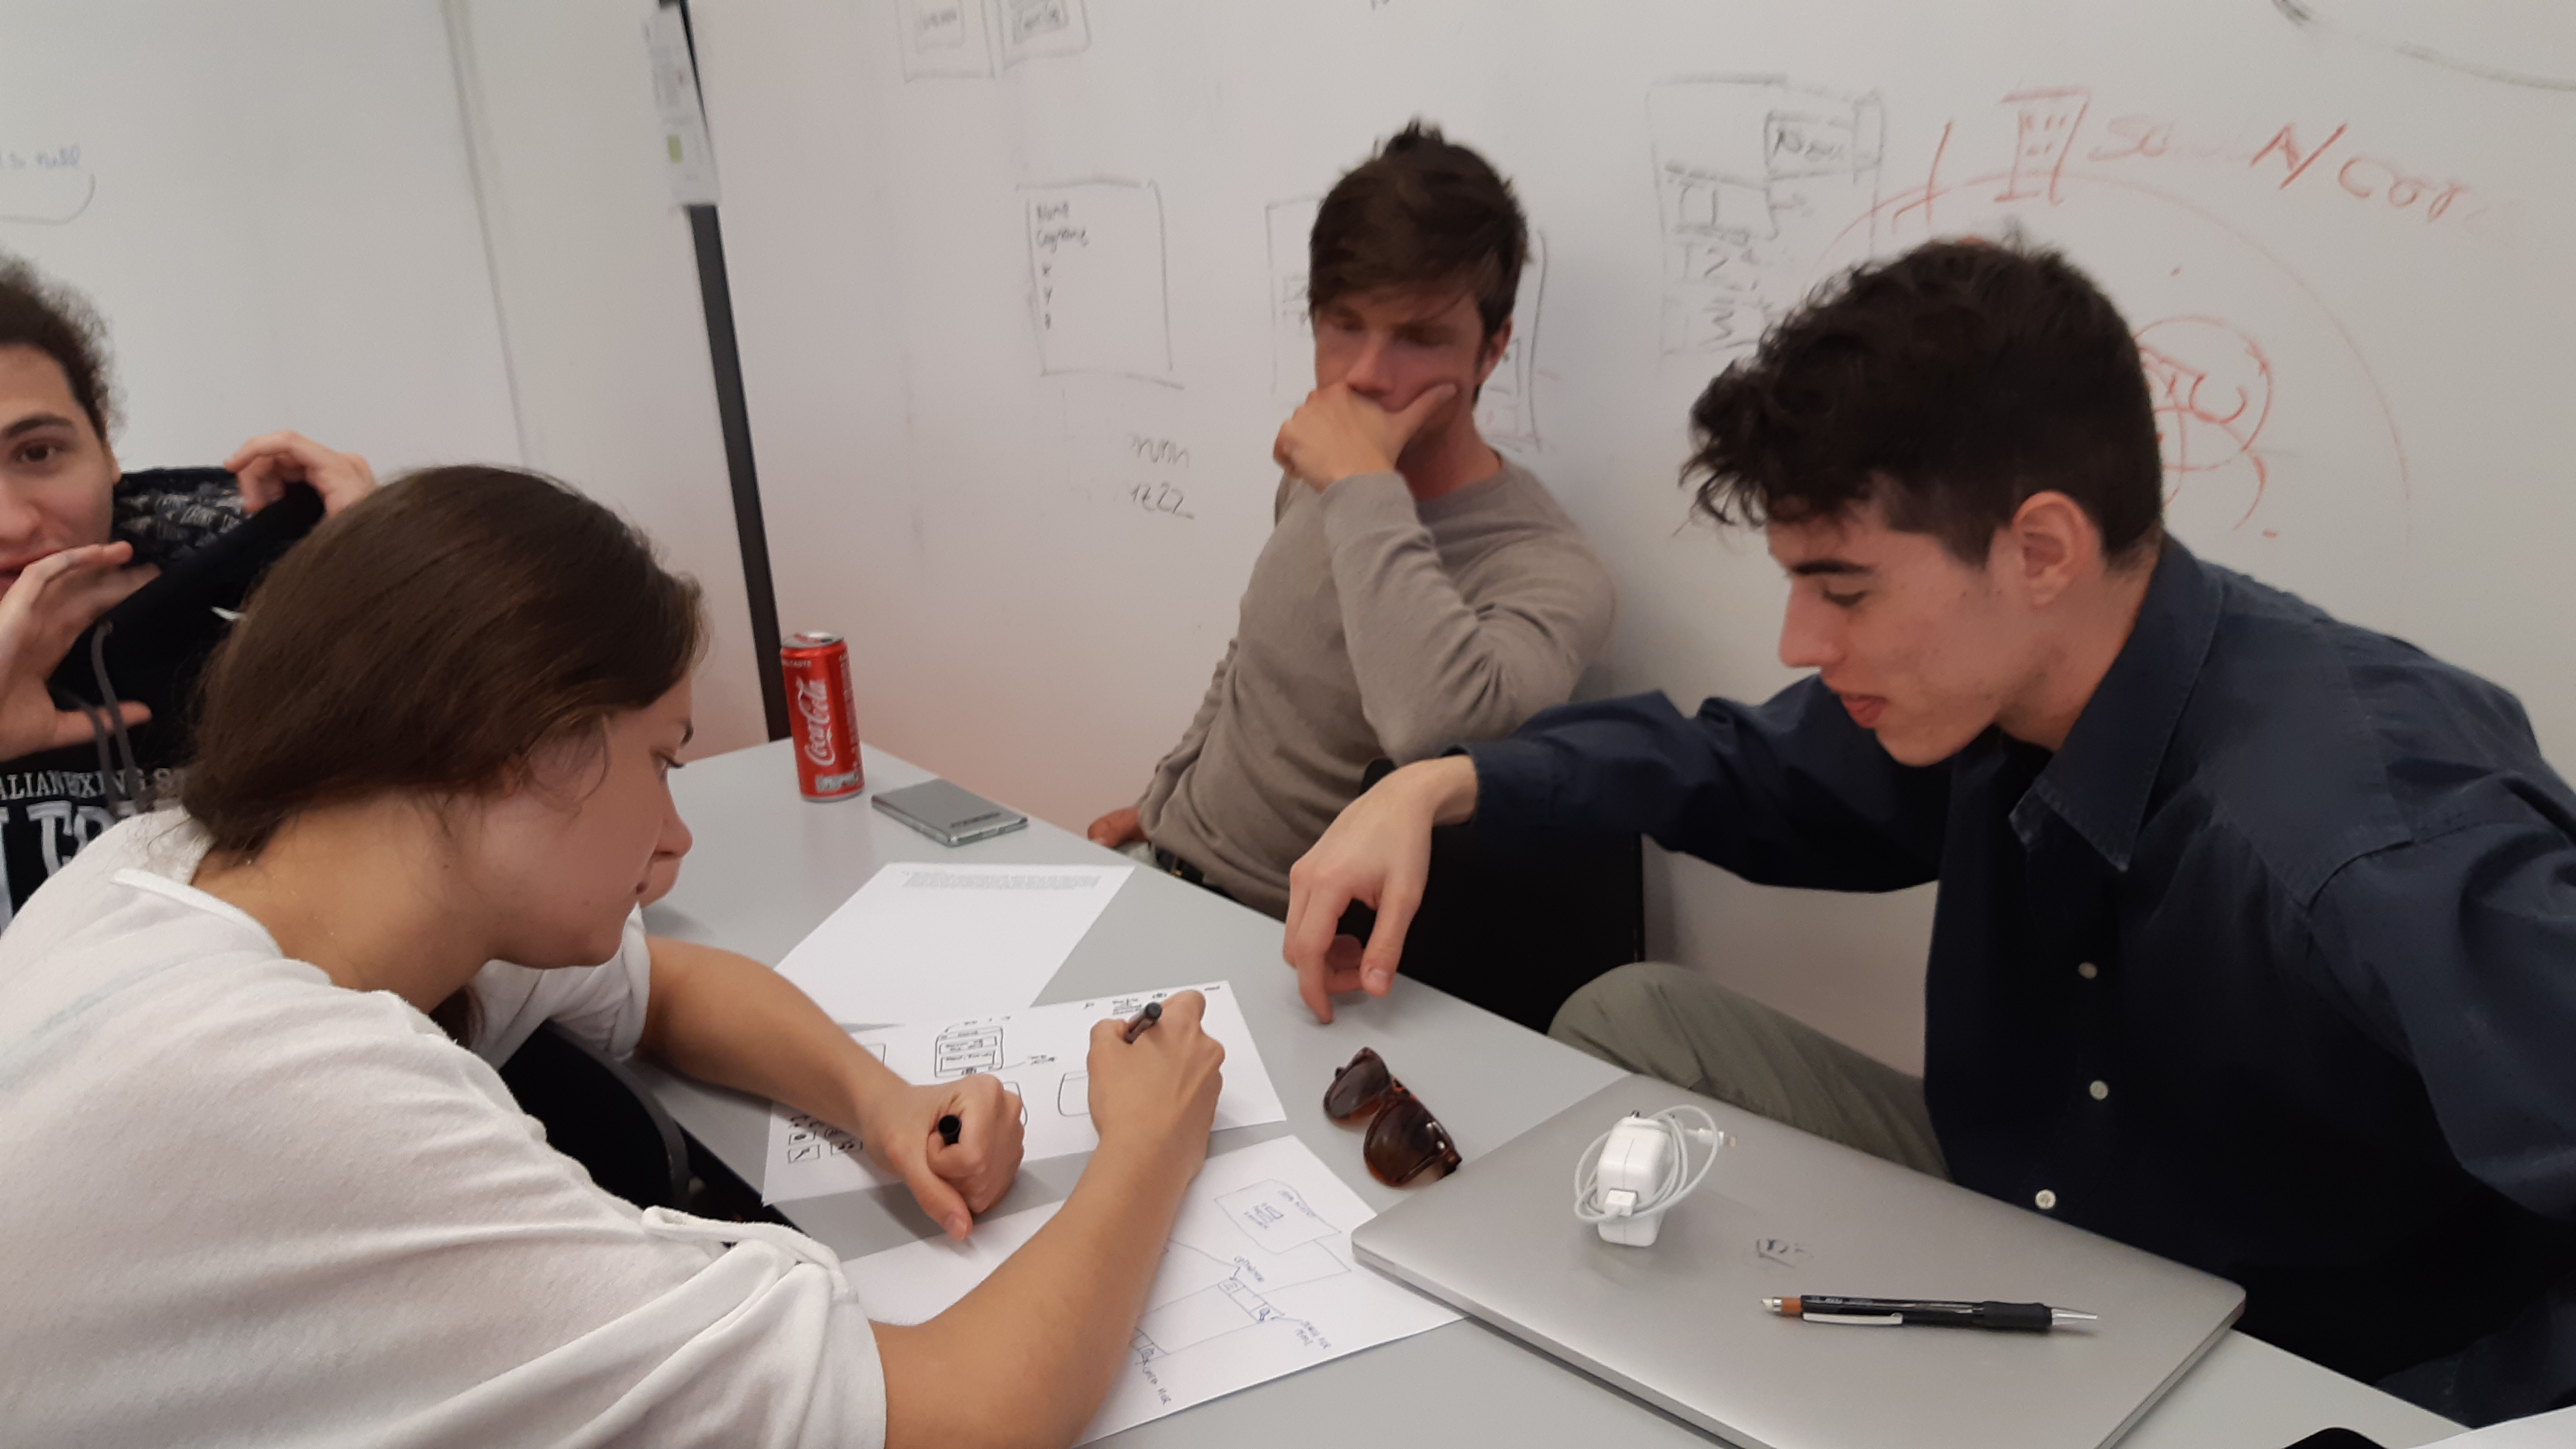
\includegraphics[width=\textwidth]{../images/group2.jpg}
       		\caption{Our team at work}
        		\label{group2}
	\end{figure}
	
	
\section{Sketches}
	
	Show scans of selected sketches.
	
	\begin{figure}[H]
        		\centering
       		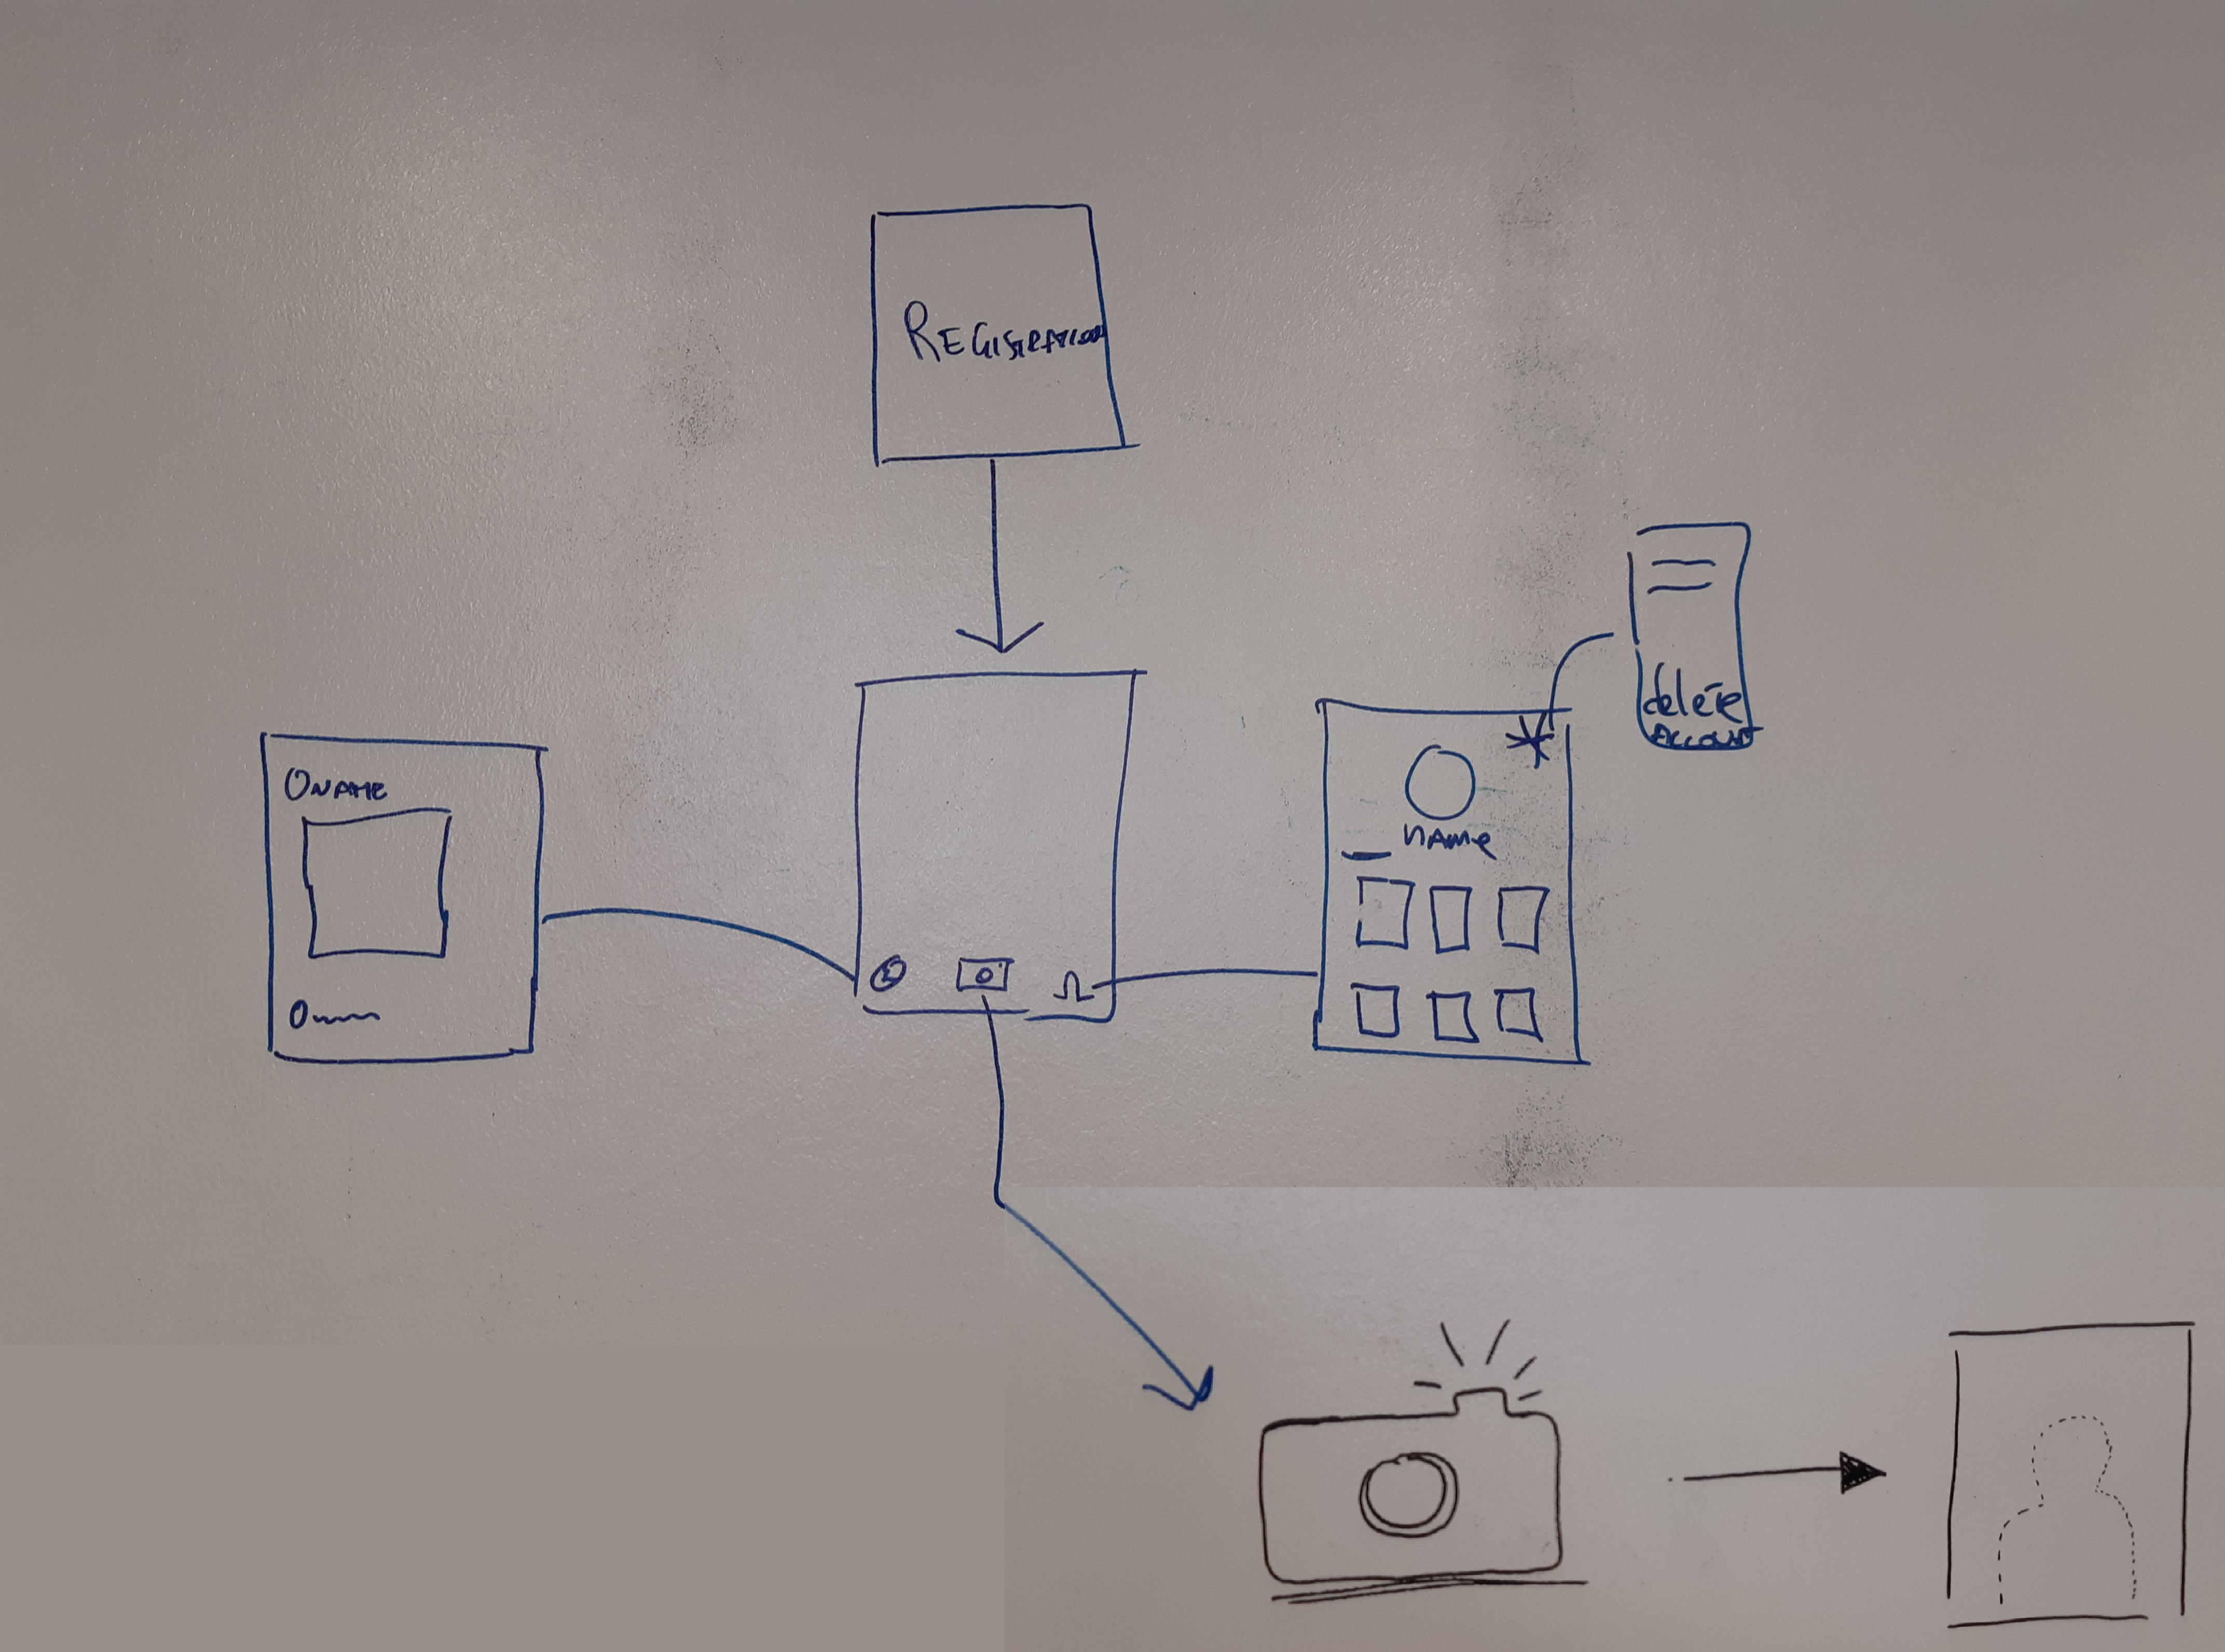
\includegraphics[width=\textwidth]{../images/design1.jpg}
       		\caption{The very first sketch}
        		\label{sketch1}
	\end{figure}
	
	\begin{figure}[H]
        		\centering
       		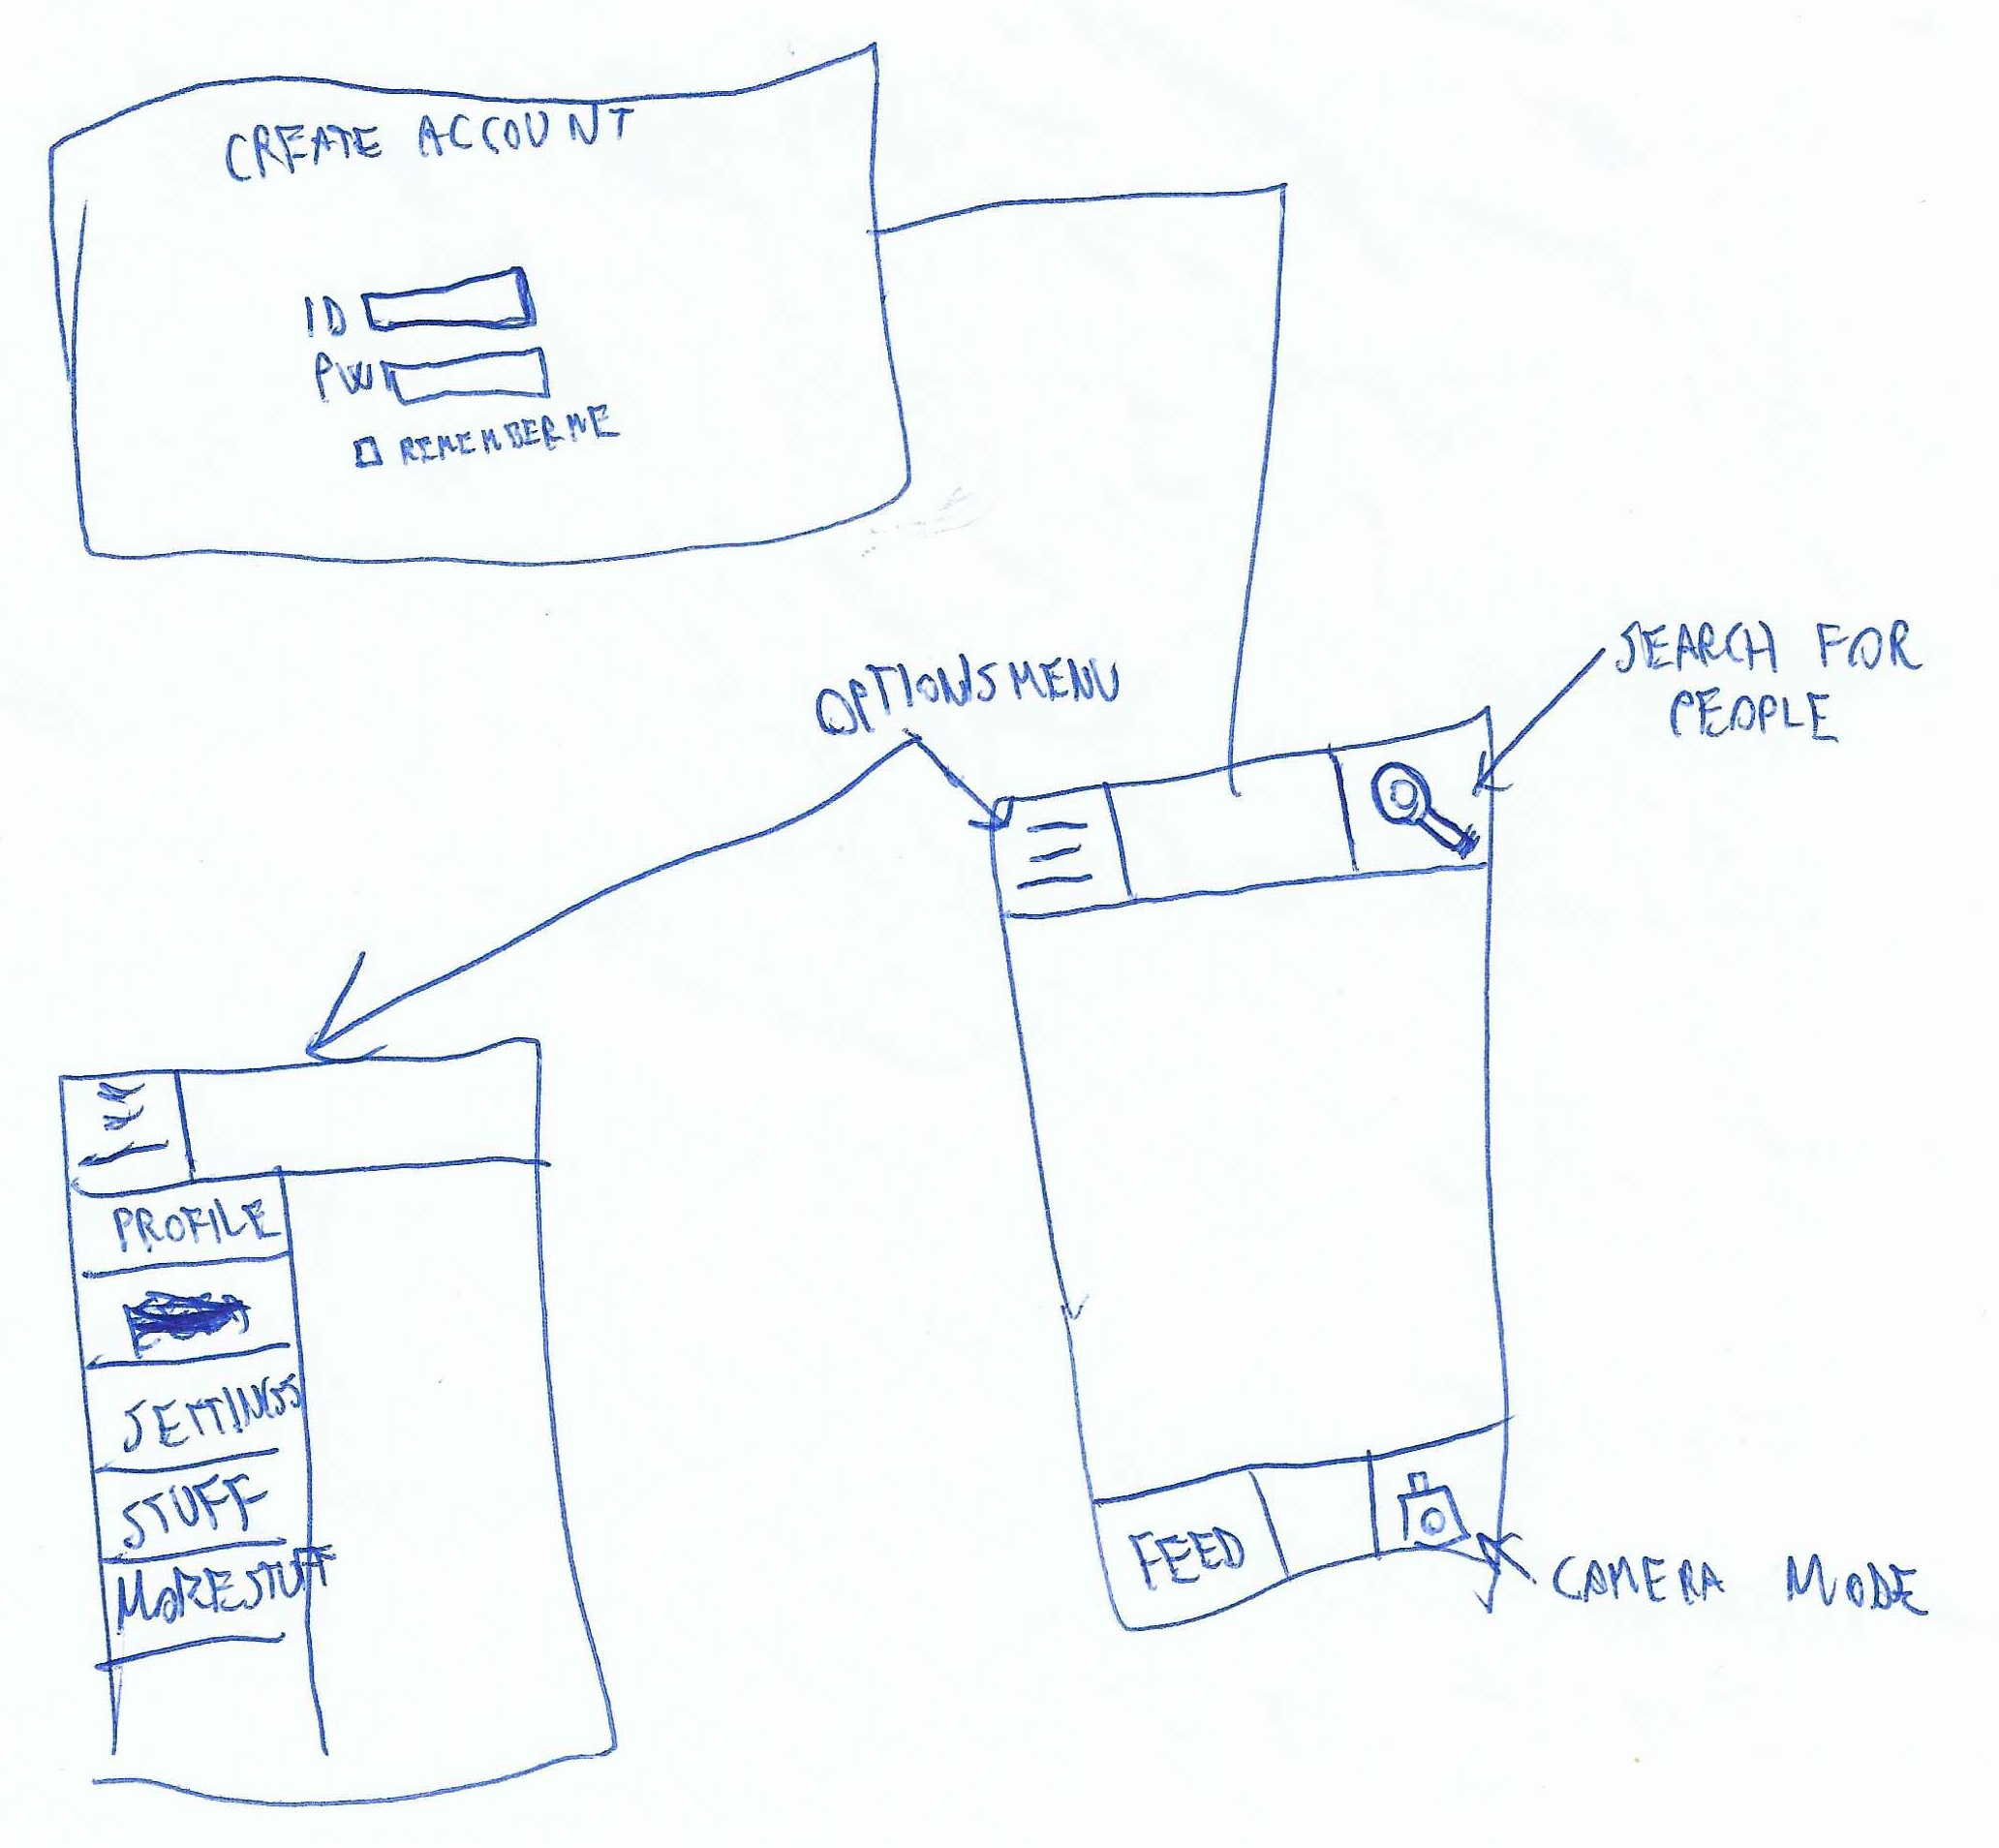
\includegraphics[width=\textwidth]{../images/design2.jpg}
       		\caption{The basic idea}
        		\label{sketch2}
	\end{figure}
	
	\begin{figure}[H]
        		\centering
       		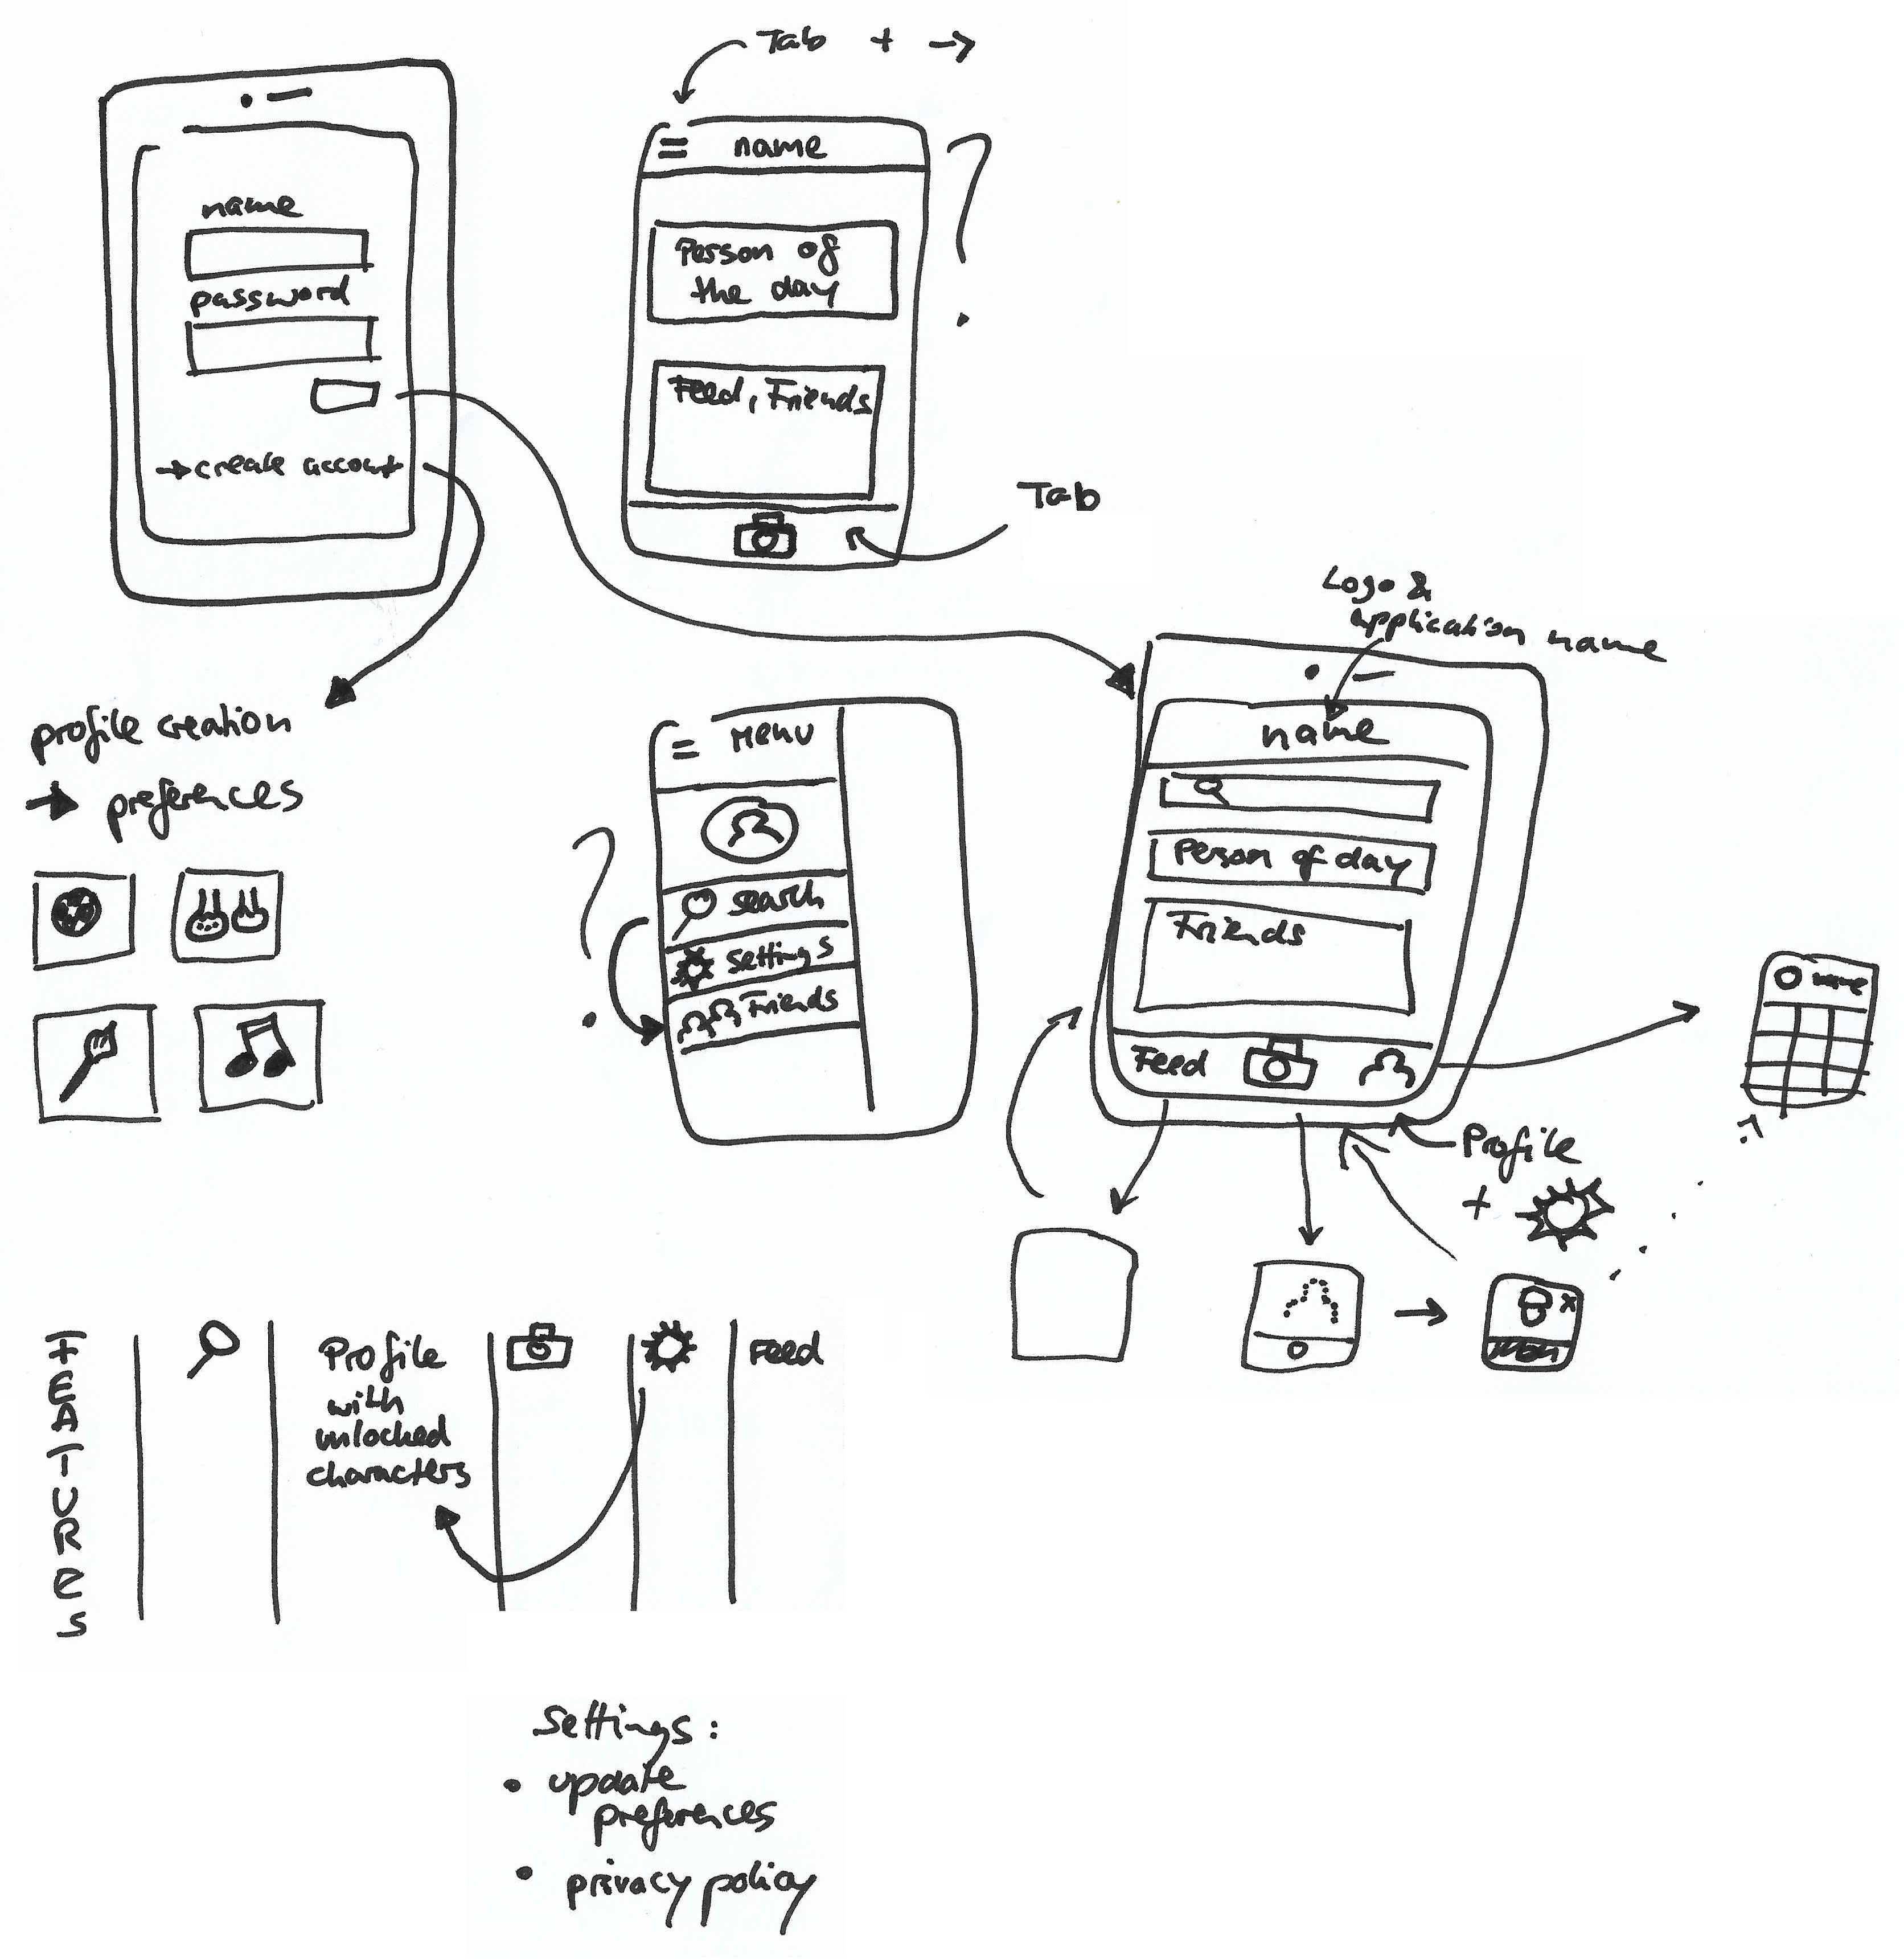
\includegraphics[width=\textwidth]{../images/design3.jpg}
       		\caption{Adding complexity}
        		\label{sketch3}
	\end{figure}
	
	
\section{Storyboard}
	
	Show your storyboard (probably as scans or photos), and explain the process very briefly. Explain the frame that shows the transition from one adjacent frame to another.
	
	\begin{figure}[H]
        		\centering
       		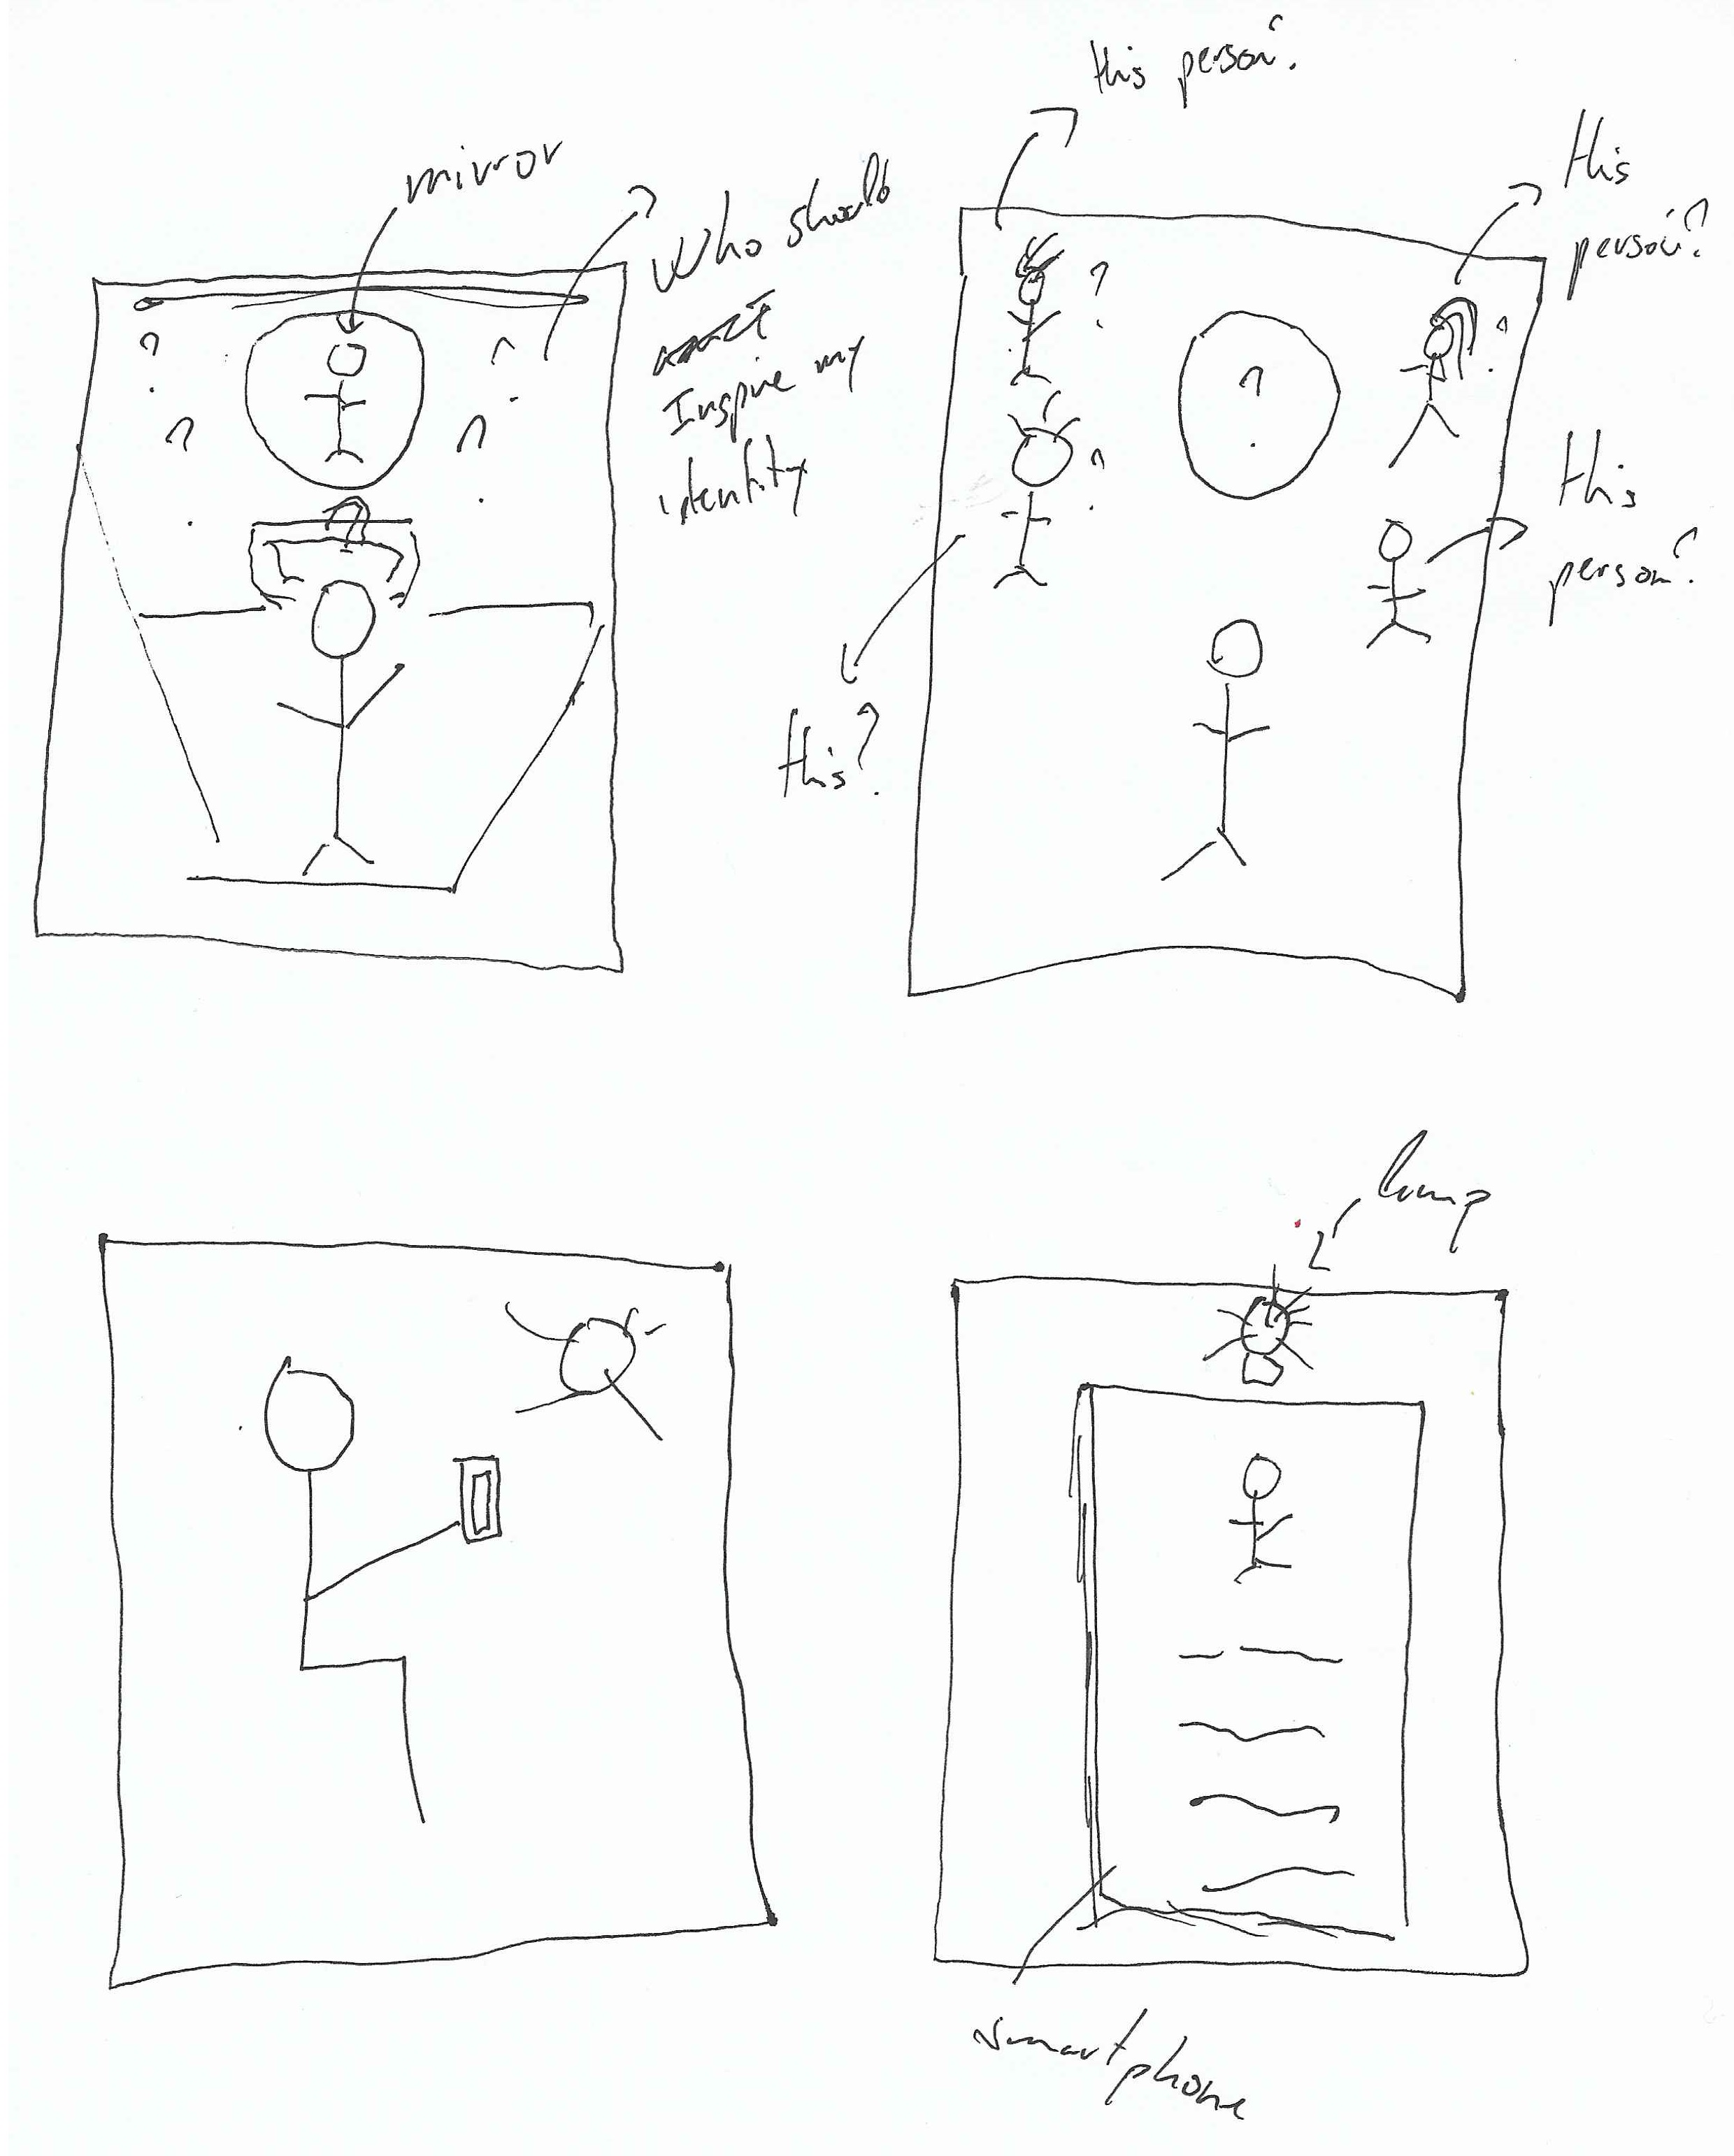
\includegraphics[width=\textwidth]{../images/story1.jpg}
       		\caption{The First Story (by Filippo)}
        		\label{story1}
	\end{figure}
	
	\begin{figure}[H]
        		\centering
       		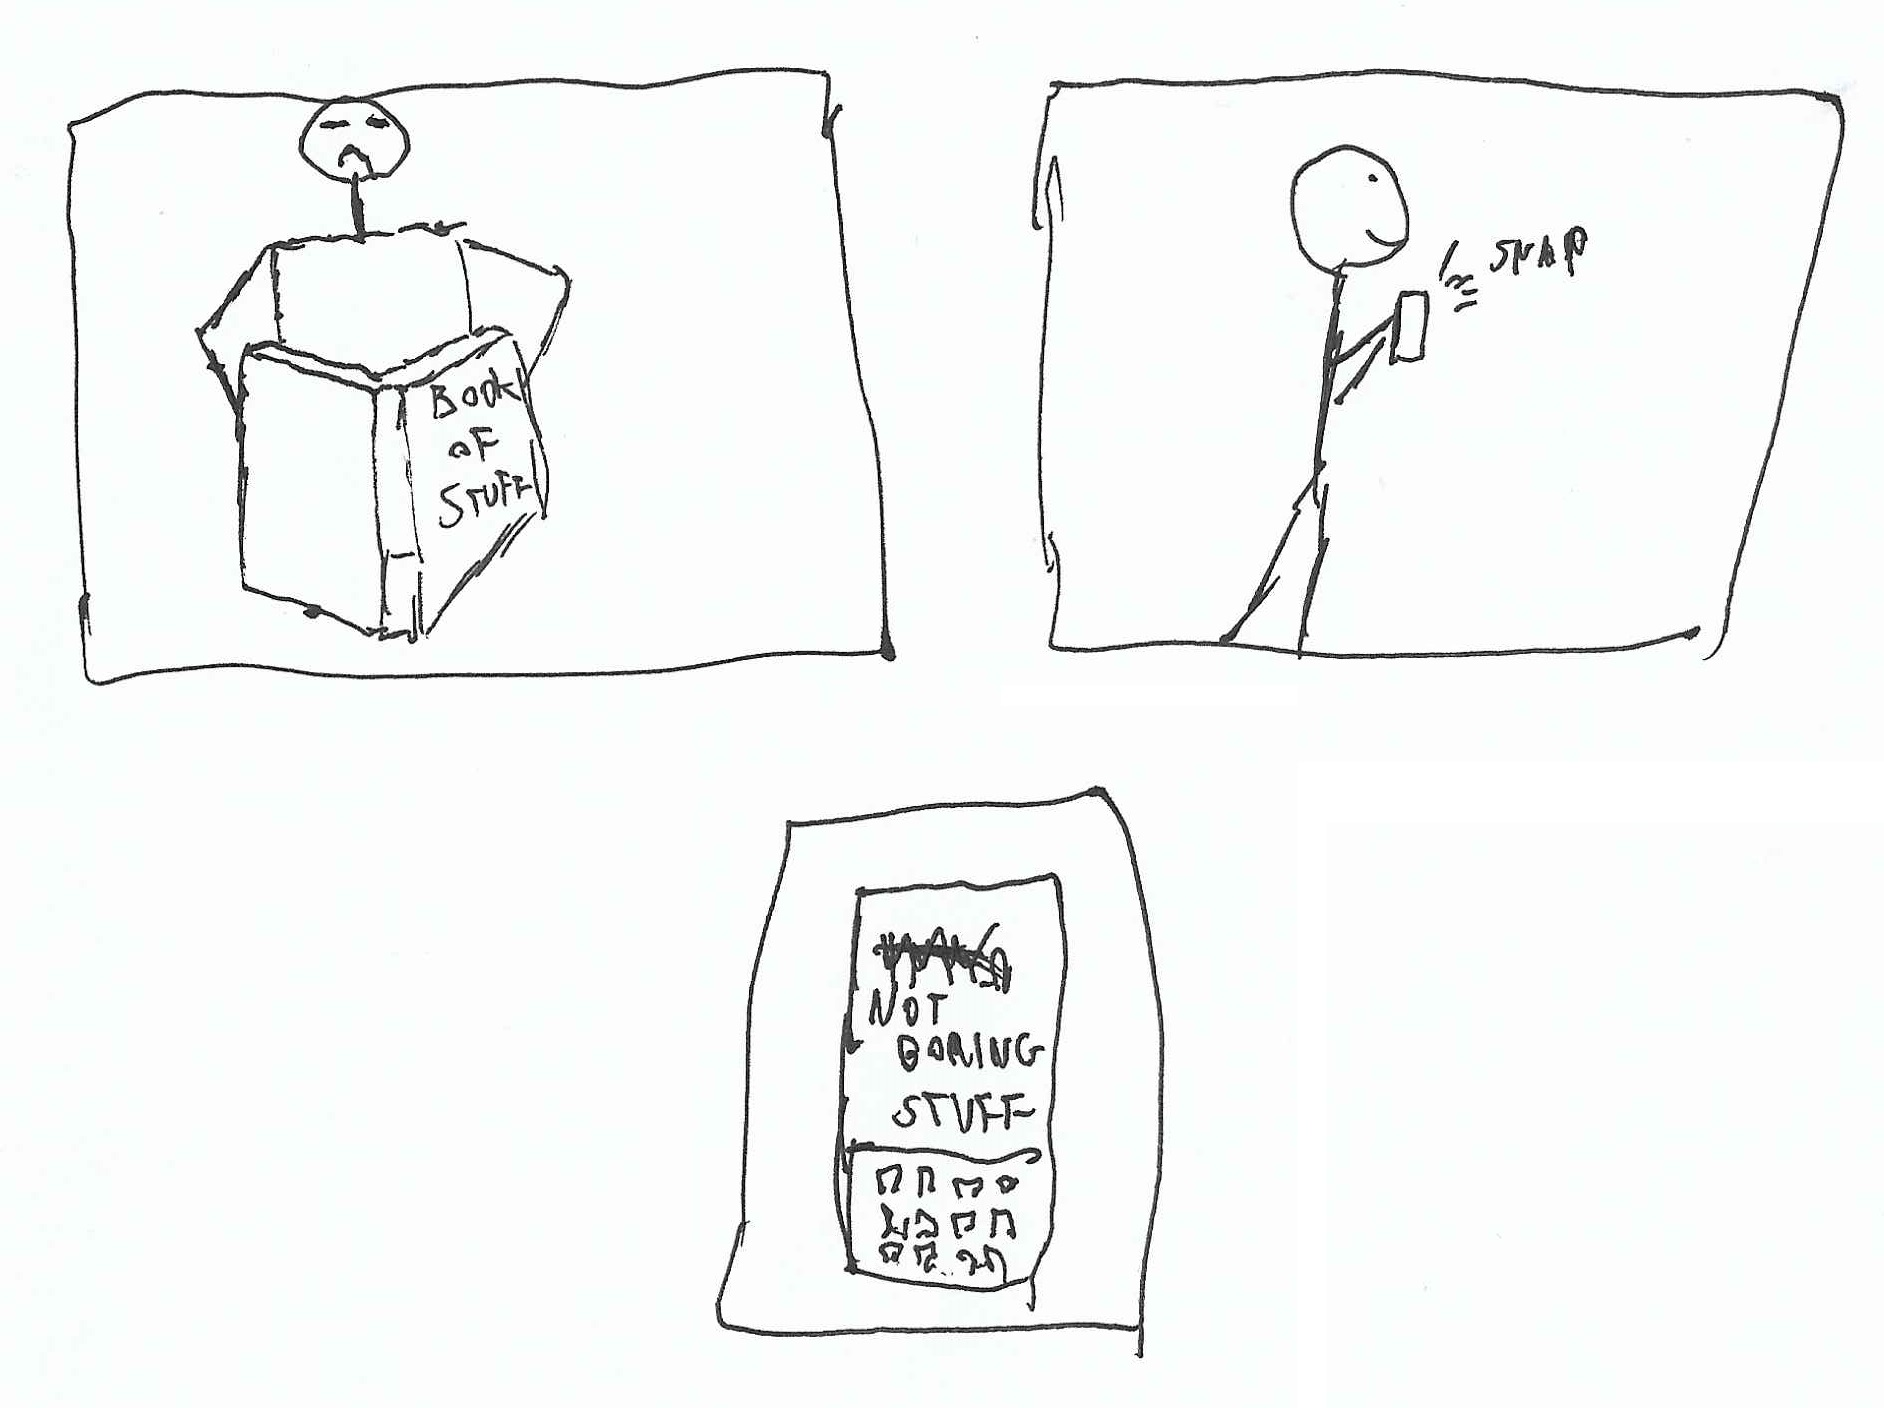
\includegraphics[width=\textwidth]{../images/story2.jpg}
       		\caption{The Second Story (by Tommaso)}
        		\label{story2}
	\end{figure}
	
	\begin{figure}[H]
        		\centering
       		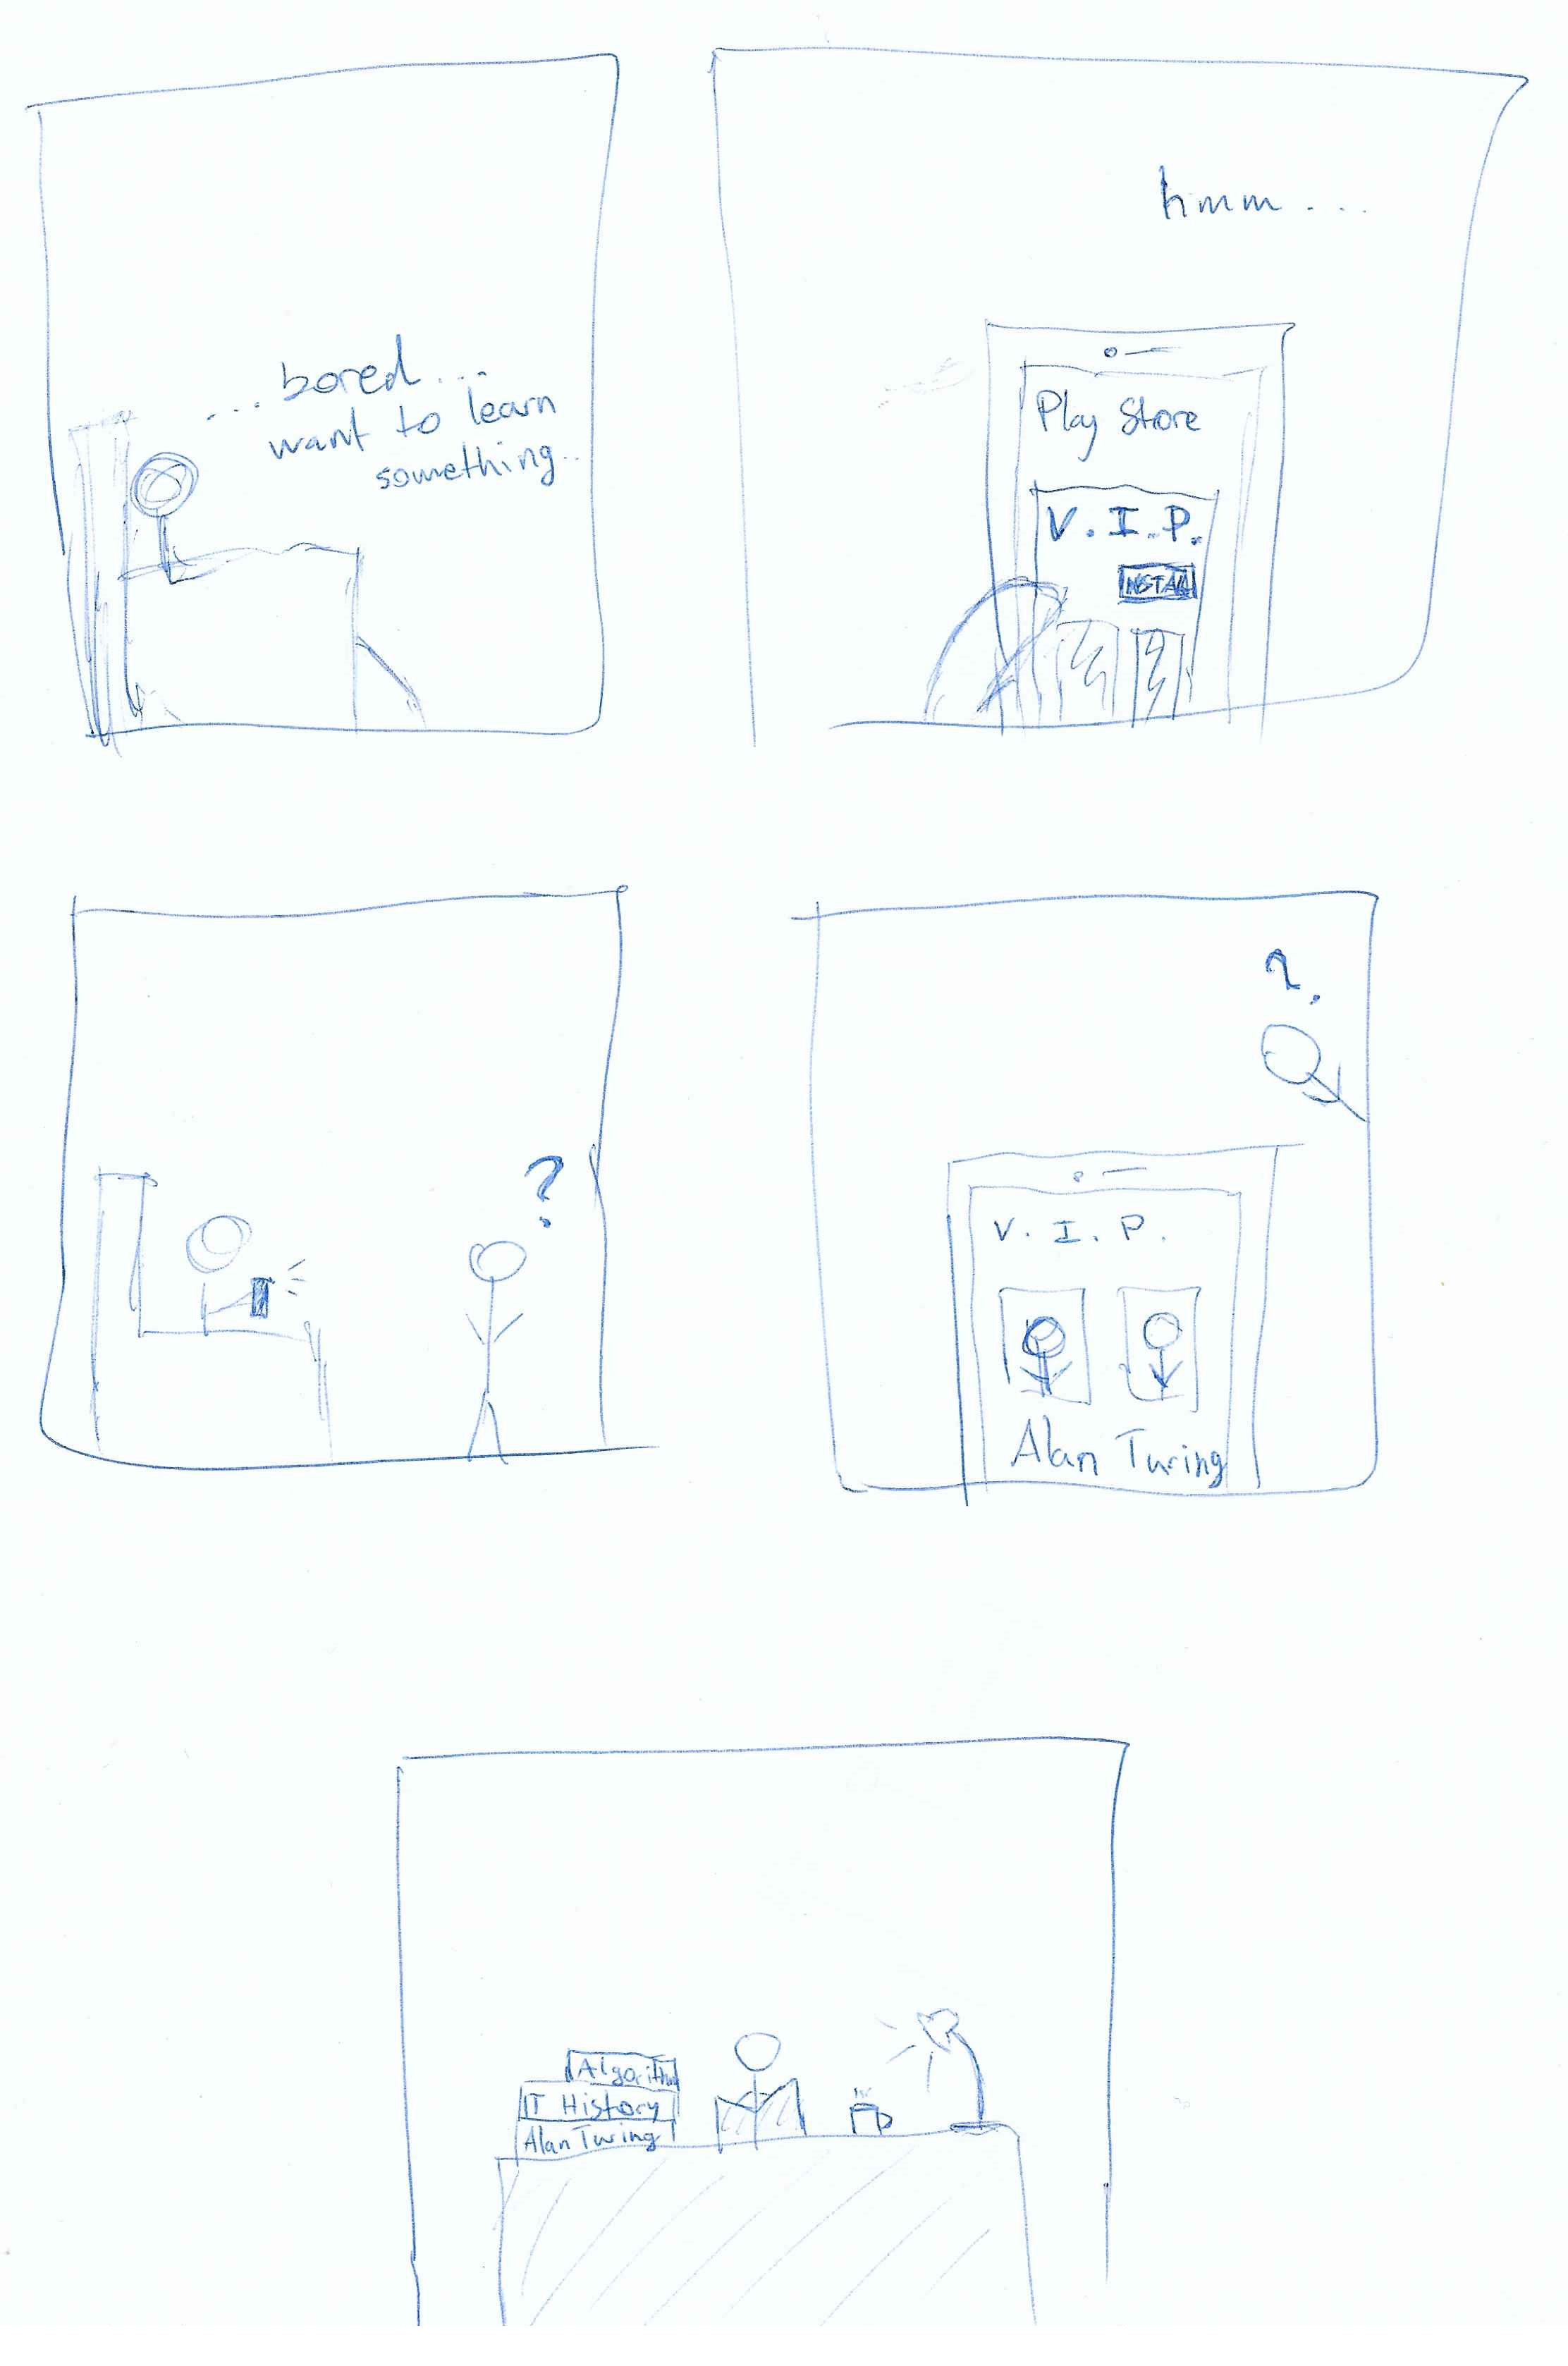
\includegraphics[width=\textwidth]{../images/story3.jpg}
       		\caption{The Third Story (by Stefano)}
        		\label{story3}
	\end{figure}
	
	%Jacopo' story here
	

\section{Wireframe}

	Make a wireframe representation of a set of related intermediate screen designs, corresponding to the usage/design scenario you used for the storyboard above.  Show screen layout and navigation.
	
	%Balsamiq exports?
	
	
\section{Conclusions}

	Write conclusions about what you have learned and progress in your project.
	

\end{document}